\section{122 - MAT - AN 3.3, AN 4.3, FA 1.4 - Aufzugsfahrt - Matura 18/19 2. NT}

\begin{langesbeispiel} \item[6] %PUNKTE DES BEISPIELS
Die Geschwindigkeiten von Personenaufzügen können sich je nach Bauart und Gebäudehöhe sehr stark unterscheiden.

Die nachstehende Abbildung zeigt das Zeit-Beschleunigung-Diagramm für eine 20\,s dauernde Aufzugsfahrt. Zu Beginn und am Ende der Fahrt steht der Aufzug still. Die Zeit $t$ wird in Sekunden, die Beschleunigung $a(t)$ in m/s$^2$ angegeben. Die Beschleunigungswerte wurden mithilfe eines Sensors ermittelt und der Verlauf der Beschleunigung wurde mit einer differenzierbaren Funktion $a$ modelliert.

\begin{center}
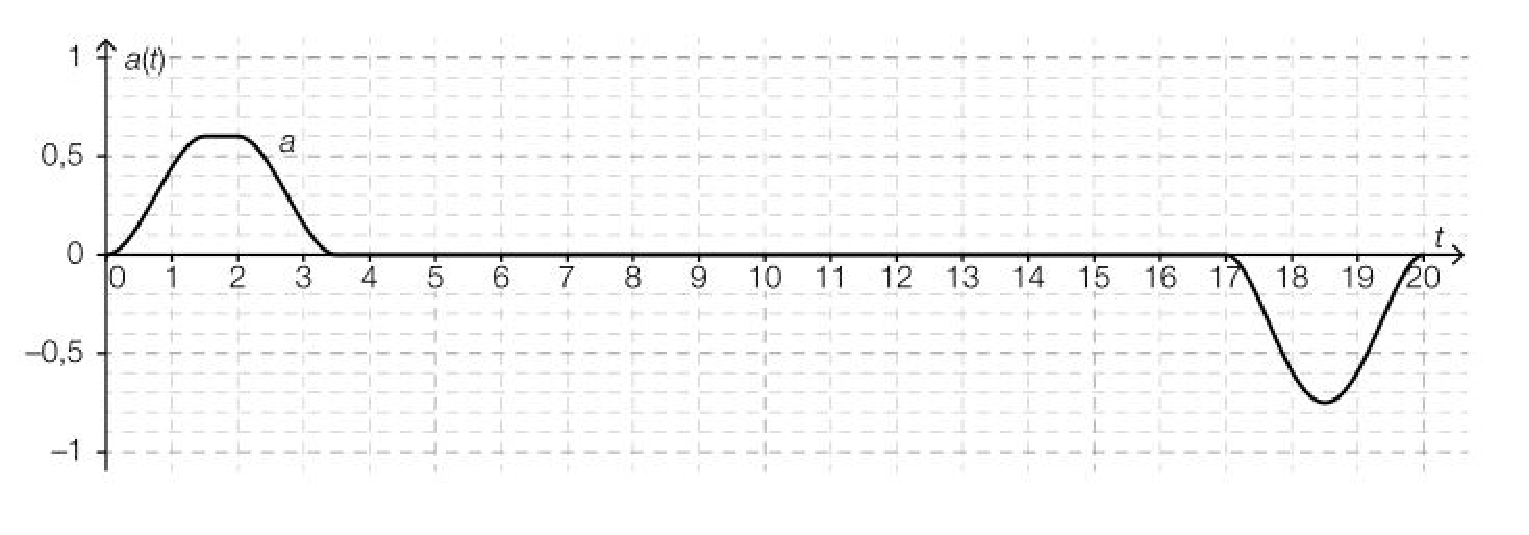
\includegraphics[width=0.8\textwidth]{../_database/Bilder/122_zug.eps}
\end{center}%Aufgabentext

\begin{aufgabenstellung}
\item %Aufgabentext

\ASubitem{Gib für jeden im Folgenden genannten Abschnitt der dargestellten Aufzugsfahrt das entsprechende Zeitintervall an.\vspace{0,3cm}
	
	Aufzug bremst ab: \antwort[\rule{3cm}{0.3pt}]{$[17\,\text{s};20\,\text{s}]$}\vspace{0,3cm}
	
	Aufzug fährt mit konstanter Geschwindigkeit: \antwort[\rule{3cm}{0.3pt}]{$[3,5\,\text{s}; 17\,\text{s}]$}} %Unterpunkt1
	
Kim behauptet, dass die Geschwindigkeit des Aufzugs im Intervall $[1,5\,\text{s}; 2\,\text{s}]$ konstant bleibt.	
	
\Subitem{Gib an, ob Kim recht hat, und begründe deine Entscheidung.} %Unterpunkt2

\item %Aufgabentext

\Subitem{Ermittle anhand der gegebenen Abbildung näherungsweise die Höchstgeschwindigkeit $v_\text{max}$ während der dargestellten Aufzugsfahrt.} %Unterpunkt1

Der Graph der Funktion $a$ schließt mit der $t$-Achse in den Zeitintervallen $[0;3,5]$ und $[17;20]$ jeweils ein Flächenstück ein.

\Subitem{Begründe, warum im gegebenen Kontext die Inhalte dieser beiden Flächenstücke gleich groß sein müssen.} %Unterpunkt2

\item Ein Produzent von Aufzugsanlagen plant die Herstellung eines neuen Aufzugs.\\
	Die Beschleunigung dieses Aufzugs wird in den ersten 3 Sekunden durch die differenzierbare Funktion $a_1$: $[0;3]\rightarrow \mathbb{R}$ mit
	
	$a_1(t)=\begin{cases}
	0,6\cdot t^2\cdot(3-2\cdot t)&\text{für}\quad 0\leq 1<1\\
	0,6&\text{für}\quad 1\leq t<2\\	
	0,6\cdot(t-3)^2\cdot(2\cdot t-3)&\text{für}\quad 2\leq t\leq 3
	\end{cases}$
	
	beschrieben ($t$ in s, $a_1(t)$ in m/s$^2$).%Aufgabentext

\Subitem{Berechne die Geschwindigkeitszunahme dieses Aufzugs im Zeitintervall $[0;3]$.} %Unterpunkt1

Für den Verlauf der Fahrt müssen bestimmte Bedingungen für die Beschleunigung eingehalten werden. Der sogenannte \textit{Ruck}, die momentane Änderungsrate der Beschleunigung, soll bei einer Fahrt mit einem Aufzug Werte zwischen $-1$\,m/s$^3$ und 1\,m/s$^3$ annehmen.

\Subitem{Überprüfe, ob dieser Aufzug bei $t=1$ die angeführten Bedingungen für den Ruck einhält.} %Unterpunkt2

\end{aufgabenstellung}

\begin{loesung}
\item \subsection{Lösungserwartung:} 

\Subitem{Der Aufzug bremst ab: $[17\,\text{s}; 20\,\text{s}]$
	
	Aufzug fährt mit konstanter Geschwindigkeit: $[3,5\,\text{s}; 17\,\text{s}]$} %Lösung von Unterpunkt1
\Subitem{Kim hat nicht recht, da die Beschleunigung in diesem Zeitintervall konstant und positiv ist und somit die Geschwindigkeit gleichmäßig (linear) zunimmt.} %%Lösung von Unterpunkt2

\setcounter{subitemcounter}{0}
\subsection{Lösungsschlüssel:}
 
\Subitem{Ein Ausgleichspunkt für die Angabe der beiden richtigen Zeitintervalle.

		Abweichungen von bis zu $\pm 0,3$\,s bei den Intervallgrenzen sind als richtig zu werten.} %Lösungschlüssel von Unterpunkt1
\Subitem{Ein Punkt für eine richtige Beschreibung.} %Lösungschlüssel von Unterpunkt2

\item \subsection{Lösungserwartung:} 

\Subitem{$\dfrac{3,5+0,5}{2}\cdot 0,6=1,2 \Rightarrow v_\text{max}\approx 1,2$\,m/s} %Lösung von Unterpunkt1
\Subitem{Die Inhalte der beiden Flächenstücke müssen gleich groß sein, da die Geschwindigkeitszunahme während der Beschleunigungsphase gleich groß wie die Geschwindigkeitsabnahme während des Abbremsvorgangs sein muss.} %%Lösung von Unterpunkt2

\setcounter{subitemcounter}{0}
\subsection{Lösungsschlüssel:}
 
\Subitem{Ein Punkt für die richtige Lösung, wobei die Einheit "`m/s"' nicht angeführt sein muss.

		Toleranzintervall: $[1\,\text{m/s}; 1,4\,\text{m/s}]$} %Lösungschlüssel von Unterpunkt1
\Subitem{Ein Punkt für eine richtige Begründung.} %Lösungschlüssel von Unterpunkt2

\item \subsection{Lösungserwartung:} 

\Subitem{$\displaystyle\int^1_0 0,6\cdot t^2\cdot(3-2\cdot t)\,\text{d}t+\displaystyle\int^2_1 0,6\,\text{d}t+\displaystyle\int^3_2 0,6\cdot(t-3)^2\cdot(2\cdot t-3)\,\text{d}t=1,2$
	
	Im Zeitintervall $[0;3]$ beträgt die Geschwindigkeitszunahme $1,2$\,m/s.} %Lösung von Unterpunkt1
\Subitem{mögliche Vorgehensweise:\\
	$a'_1(t)=0$ für alle $t\in[1;2) \Rightarrow a'_1(1)=0$
	
	Zum Zeitpunkt $t=1$ beträgt die momentane Änderungsrate der Beschleunigung $0$\,m/s$^3$.\\
	Die angeführten Bedingungen sind bei $t=1$ eingehalten.} %%Lösung von Unterpunkt2

\setcounter{subitemcounter}{0}
\subsection{Lösungsschlüssel:}
 
\Subitem{Ein Punkt für die richtige Lösung, wobei die Einheit "`m/s"' nicht angeführt sein muss.

		Toleranzintervall: $[1,1; 1,3]$\\
		Die Aufgabe ist auch dann als richtig gelöst zu werten, wenn bei korrektem Ansatz das Ergebnis aufgrund eines Rechenfehlers nicht richtig ist.} %Lösungschlüssel von Unterpunkt1
\Subitem{Ein Punkt für einen richtigen rechnerischen Nachweis.} %Lösungschlüssel von Unterpunkt2

\end{loesung}

\end{langesbeispiel}